\documentclass[10pt,a4paper]{article}
\usepackage[utf8]{inputenc}
\usepackage[T1]{fontenc}
\usepackage[brazil]{babel}
\usepackage{geometry}
\geometry{a4paper, left=1.8cm, right=1.8cm, top=1.8cm, bottom=1.8cm}
\usepackage{amsmath,amssymb,amsfonts}
\usepackage{booktabs}
\usepackage{graphicx}
\usepackage{float}
\usepackage{hyperref}
\usepackage{fancyhdr}
\usepackage{array}
\usepackage{caption}

\pagestyle{fancy}
\fancyhf{}
\fancyhead[L]{\small IFES -- Campus Serra}
\fancyhead[C]{\small Probabilidade e Estatística I -- Máquina Estatística}
\fancyhead[R]{\small Trabalho I -- 2026/2}
\fancyfoot[L]{\footnotesize Simulador acadêmico - somente créditos fictícios}
\fancyfoot[R]{\footnotesize Página \thepage}
\renewcommand{\headrulewidth}{0.4pt}
\renewcommand{\footrulewidth}{0.4pt}

\hypersetup{
    colorlinks=true,
    linkcolor=blue,
    citecolor=blue,
    urlcolor=blue
}

\begin{document}

\begin{center}
    {\bfseries Instituto Federal do Espírito Santo -- Campus Serra}\\
    {\small Bacharelado em Sistemas de Informação | Probabilidade e Estatística I -- Trabalho I (2026/2)}\\[6pt]
    {\Large \bfseries MÁQUINA ESTATÍSTICA: PROBABILIDADE, APOSTAS E PENSAMENTO CRÍTICO}\\[4pt]
    {\small \textbf{Professor:} Fidelis Zanetti de Castro \quad|\quad \textbf{Entrega:} 29 de outubro de 2026 \quad|\quad \textbf{Aviso:} \textit{Simulador acadêmico - somente créditos fictícios}}
\end{center}
\hrule
\vspace{8pt}

\section{Contexto, problemática e situação das fontes no tempo}

A rápida difusão das apostas digitais no Brasil conectou algoritmos de sorteio instantâneo, meios de pagamento imediato (como o Pix), publicidade intensiva por influenciadores digitais e uso contínuo do telefone celular. Entre os produtos de maior apelo visual destacam-se as máquinas virtuais de rolos (\textit{online slots}), popularmente associadas ao chamado ``jogo do tigrinho'' \cite{ribas2025,pacete2024}. Embora animações, efeitos sonoros e vitórias ocasionais tornem cada rodada intuitiva, a interface gráfica não explicita ao usuário a probabilidade real de obter um prêmio nem o comportamento financeiro acumulado de repetir a aposta centenas de vezes. Este trabalho investiga a pergunta central proposta na especificação: \textbf{como ganhos ocasionais podem coexistir com uma perda esperada para o jogador, e o que essa diferença nos ajuda a compreender sobre as apostas na sociedade?}

Para responder a essa questão com rigor metodológico, é indispensável separar dois planos analíticos: (i) a \textbf{demonstração matemática e computacional} de uma máquina didática com regras públicas (Seções 2 e 3), que descreve propriedades exatas do modelo probabilístico e resultados de participantes virtuais com créditos fictícios; e (ii) a \textbf{análise documental e epidemiológica} sobre saúde pública, orçamento familiar e regulação estatal (Seção 4), uma vez que simulações computacionais não medem prevalência clínica de transtornos nem estimam o impacto macroeconômico nacional.

\paragraph{Evolução regulatória e distinção epistemológica das fontes (2023--setembro de 2026).}
Em 29 de dezembro de 2023, a \textbf{Lei nº 14.790/2023} \cite{lei14790} (norma legal publicada) regulamentou as apostas de quota fixa em eventos esportivos e jogos on-line. Em 19 de maio de 2026, o \textbf{Tribunal de Contas da União (Acórdão nº 1296/2026 -- Plenário)} \cite{tcu2026} (auditoria institucional) apontou falhas de coordenação governamental e limitações técnicas no bloqueio de operadores clandestinos. Em \textbf{25 de setembro de 2026}, foi editada a \textbf{Medida Provisória nº 1.394/2026} \cite{mp1394,ms2026} (norma publicada com força de lei imediata), estabelecendo a proibição da exploração, oferta, intermediação e publicidade de apostas de quota fixa e jogos on-line no país, preservadas as demais modalidades lotéricas autorizadas em lei. Em \textbf{28 de setembro de 2026}, a União ajuizou ação contra 17 plataformas pedindo no mínimo R\$ 1 bilhão por danos morais coletivos e ressarcimento ao SUS \cite{richter2026}, enquanto ANJL e IBJR acionaram o STF solicitando a suspensão da MP \cite{pontes2026}. Tais requerimentos constituem \textbf{pedidos e argumentos das partes}, não equivalendo a condenação judicial nem a decisão definitiva do STF. Do mesmo modo, a Tabela \ref{tab:contexto} distingue as três grandes cifras nacionais, que não podem ser somadas por medirem conceitos, universos e períodos distintos.

\begin{table}[H]
\centering
\caption{Distinção conceitual, temporal e metodológica entre as medidas macroeconômicas e epidemiológicas de referência.}
\label{tab:contexto}
\footnotesize
\begin{tabular}{p{2.8cm}p{3.6cm}p{3.0cm}p{6.8cm}}
\toprule
\textbf{Indicador} & \textbf{Fonte e Gênero} & \textbf{Período / Universo} & \textbf{Interpretação Correta e Limites} \\
\midrule
R\$ 18--21 bilhões mensais & Banco Central (NT 513/2024; EE 119/2024) \cite{bcb2024} -- Nota técnica & Jan--Ago 2024; pessoas físicas via Pix & Mede \textbf{transferências brutas} enviadas via Pix. Não desconta prêmios sacados nem reapostas; não equivale à perda líquida. \\
R\$ 17,4 bilhões no semestre & TCU (Acórdão 1296/2026) \cite{tcu2026} -- Auditoria institucional & 1º sem. 2025; mercado autorizado (SPA/MF) & Mede a \textbf{receita bruta de jogos (GGR)}: valores apostados menos prêmios pagos. Difere de depósitos e de lucro líquido. \\
R\$ 38,8 bilhões anuais (R\$ 30,6 bi saúde) & Rosa et al. / IEPS (2025) \cite{ieps2025} -- Dossiê de pesquisa & Projeção anualizada; população afetada & Estimativa de \textbf{custos sociais} (monetários e valoração de QALYs) extrapolada de revisão britânica \cite{ohid2023} por PPC; não é conta paga pelo SUS. \\
15,8\% (IC 95\%: 10,7\%--21,6\%) & Wardle et al., \textit{Lancet Public Health} (2024) \cite{wardle2024} -- Meta-análise & Estudos internacionais; \textbf{adultos que usaram cassino/rolos on-line} & O denominador restringe-se aos \textbf{usuários da modalidade}, não representando 15,8\% de toda a população adulta brasileira. \\
\bottomrule
\end{tabular}
\begin{flushleft}
\scriptsize \textit{Fonte:} Elaboração própria a partir de Banco Central \cite{bcb2024}, TCU \cite{tcu2026}, IEPS \cite{ieps2025}, OHID/PHE \cite{ohid2023} e Wardle et al. \cite{wardle2024}.
\end{flushleft}
\end{table}

\section{Modelo da máquina didática e fundamentação matemática}

O modelo utiliza cinco símbolos discretos, $\mathcal{R} = (\text{A}, \text{B}, \text{C}, \text{D}, \text{E})$, indexados de $0$ a $4$ em cada um dos três rolos. A aposta é fixa de $1$ crédito fictício por rodada. Sorteia-se uma parada $K \in \{0, 1, 2, 3, 4\}$ uniformemente ($\Pr(K=k) = 1/5$) de forma independente para cada rolo. A coluna exibe $\mathcal{R}_K$ no topo, $\mathcal{R}_{(K+1) \bmod 5}$ no centro e $\mathcal{R}_{(K+2) \bmod 5}$ na base. Assim, as células de uma mesma coluna vertical \textbf{não são independentes} (são posições vizinhas determinadas pelo mesmo $K$), mas as três células da linha central pertencem a rolos sorteados independentemente, sendo \textbf{mutuamente independentes}.

Há $|\Omega| = 5^3 = 125$ triplas centrais equiprováveis, cada uma com probabilidade $(1/5)^3 = 1/125 = 0{,}80\%$. Apenas as cinco triplas idênticas (A--A--A, B--B--B, C--C--C, D--D--D e E--E--E) pagam prêmio bruto $P \in \{5, 10, 15, 25, 50\}$, respectivamente; as demais $120$ triplas pagam $P = 0$. Logo, $\Pr(P > 0) = 5/125 = 4{,}00\%$ e $\Pr(P = 0) = 120/125 = 96{,}00\%$. Definindo o lucro líquido por rodada como $X = P - 1$, temos:
\[
\mathbb{E}[P] = \frac{5 + 10 + 15 + 25 + 50}{125} = \frac{105}{125} = 0{,}84, \qquad \mathbb{E}[X] = \mathbb{E}[P] - 1 = 0{,}84 - 1 = -0{,}16 \text{ crédito.}
\]
A variância teórica é $\text{Var}(X) = \mathbb{E}[X^2] - (\mathbb{E}[X])^2 = 27{,}12 - 0{,}0256 = 27{,}0944$, com desvio-padrão $\sigma_X = \sqrt{27{,}0944} \approx 5{,}2052$ créditos. O Retorno ao Jogador é $\text{RTP} = \mathbb{E}[P]/1 = 84{,}00\%$ (vantagem esperada do operador de $16{,}00\%$) \cite{gc2021}.

\begin{figure}[H]
\centering
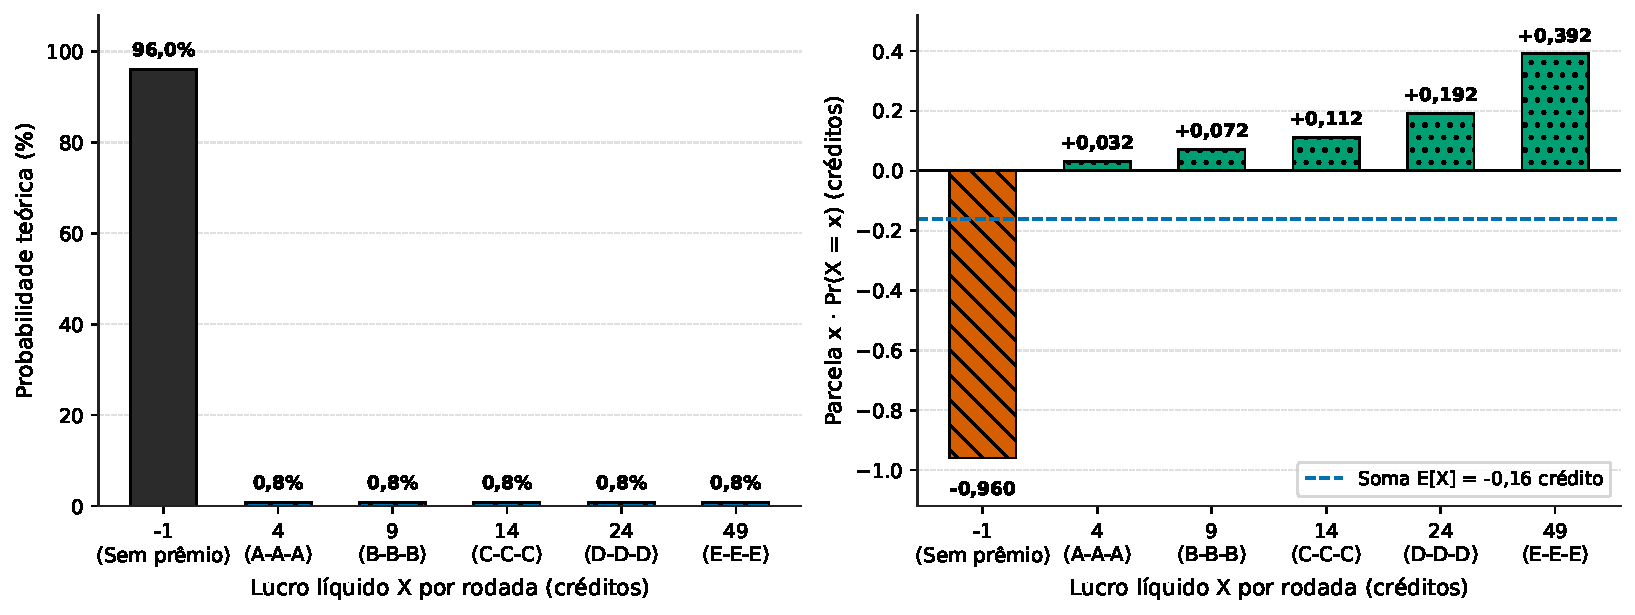
\includegraphics[width=0.98\textwidth]{resultados/graficos/fig01_modelo_teorico.pdf}
\caption{Distribuição teórica de probabilidade do lucro líquido $X$ por rodada (à esquerda) e contribuição ponderada $x \Pr(X = x)$ para a esperança matemática $\mathbb{E}[X] = -0{,}16$ crédito (à direita).}
\label{fig:modelo_teorico}
\begin{flushleft}
\scriptsize \textit{Fonte:} Elaboração própria a partir das regras públicas da Seção 5 e Tabela 1 do enunciado.
\end{flushleft}
\end{figure}

\section{Cinco experimentos computacionais: procedimento, resultados e interpretação}

As simulações foram executadas em \textbf{Python 3.12.7} (CPython 64 bits) com o gerador \texttt{random.Random(semente)} (Mersenne Twister MT19937) \cite{python_random}.

\subsection{Experimento 1 -- As frequências acompanham as probabilidades?}

Com semente \textbf{2026} e $N = 10.000$ rodadas sem regra de parada, obtiveram-se as contagens da Tabela \ref{tab:e1} (Figura \ref{fig:e1}). A soma das contagens fechou em exatamente $10.000$ ($412$ rodadas premiadas, proporção observada de $4{,}12\%$ vs.\ $4{,}00\%$ teórico). O lucro médio observado foi $\bar{X} = -0{,}1315$ crédito ($\mathbb{E}[X] = -0{,}1600$), o RTP observado foi $\widehat{\text{RTP}} = 86{,}85\%$ ($\text{RTP} = 84{,}00\%$) e o desvio-padrão amostral ($N-1$) foi $s = 5{,}2750$ créditos ($\sigma_X = 5{,}2052$). A diferença de $+0{,}0285$ crédito entre $\bar{X}$ e $-0{,}16$ corresponde a apenas $0{,}54$ erro-padrão ($\text{EP} = s/\sqrt{N} = 0{,}0528$), decorrente da variabilidade amostral binomial nas triplas B--B--B ($88$), D--D--D ($88$) e E--E--E ($81$), não autorizando qualquer alteração nos dados. Evidencia-se também que a proporção de prêmios ($4{,}12\%$) mede a frequência de eventos $\{P_i > 0\}$, enquanto o RTP ($86{,}85\%$) pondera os pagamentos pelos seus valores em créditos.

\begin{table}[H]
\centering
\caption{Distribuição teórica e resultados empíricos do Experimento 1 ($N = 10.000$ rodadas, semente 2026).}
\label{tab:e1}
\footnotesize
\begin{tabular}{lrrrrrrr}
\toprule
\textbf{Linha Central} & \textbf{$P$ (cr.)} & \textbf{$X$ (cr.)} & \textbf{Prob. Teórica} & \textbf{Esperado} & \textbf{Contagem} & \textbf{Freq. Relativa} & \textbf{Diferença} \\
\midrule
A--A--A & 5 & $+4$ & $1/125$ ($0{,}80\%$) & $80{,}0$ & 77 & $0{,}0077$ ($0{,}77\%$) & $-0{,}03$ p.p. \\
B--B--B & 10 & $+9$ & $1/125$ ($0{,}80\%$) & $80{,}0$ & 88 & $0{,}0088$ ($0{,}88\%$) & $+0{,}08$ p.p. \\
C--C--C & 15 & $+14$ & $1/125$ ($0{,}80\%$) & $80{,}0$ & 78 & $0{,}0078$ ($0{,}78\%$) & $-0{,}02$ p.p. \\
D--D--D & 25 & $+24$ & $1/125$ ($0{,}80\%$) & $80{,}0$ & 88 & $0{,}0088$ ($0{,}88\%$) & $+0{,}08$ p.p. \\
E--E--E & 50 & $+49$ & $1/125$ ($0{,}80\%$) & $80{,}0$ & 81 & $0{,}0081$ ($0{,}81\%$) & $+0{,}01$ p.p. \\
Qualquer outra tripla & 0 & $-1$ & $120/125$ ($96{,}00\%$) & $9.600{,}0$ & 9.588 & $0{,}9588$ ($95{,}88\%$) & $-0{,}12$ p.p. \\
\midrule
\textbf{Total} & --- & --- & $125/125$ ($100{,}00\%$) & $10.000{,}0$ & \textbf{10.000} & $1{,}0000$ ($100{,}00\%$) & $0{,}00$ p.p. \\
\bottomrule
\end{tabular}
\begin{flushleft}
\scriptsize \textit{Fonte:} Resultados da simulação computacional (\texttt{resultados/e1\_tabela\_frequencias.csv}).
\end{flushleft}
\end{table}

\begin{figure}[H]
\centering
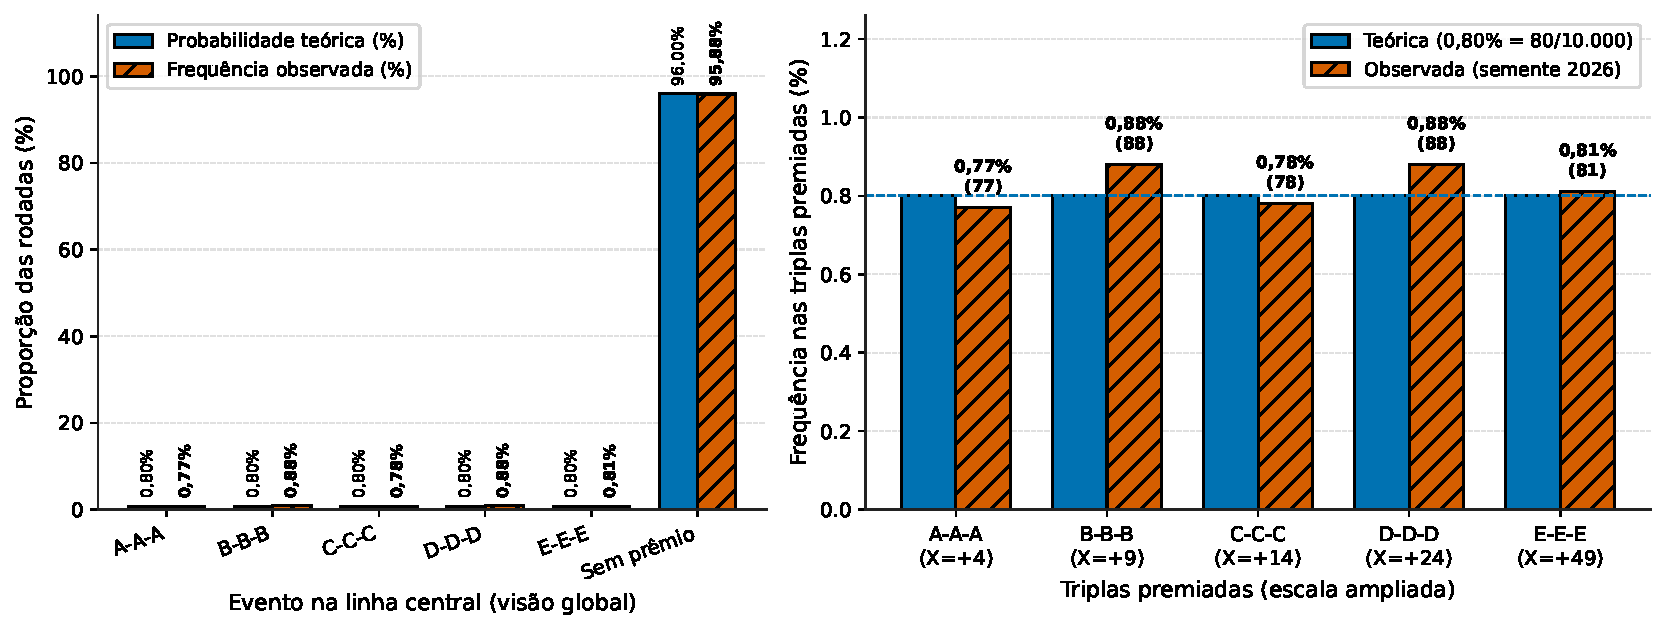
\includegraphics[width=0.98\textwidth]{resultados/graficos/fig02_e1_frequencias.pdf}
\caption{Comparação entre probabilidade teórica (\%) e frequência relativa observada (\%) no Experimento 1 ($N = 10.000$, semente 2026): visão global (à esquerda) e escala ampliada nas cinco triplas premiadas (à direita).}
\label{fig:e1}
\begin{flushleft}
\scriptsize \textit{Fonte:} Elaboração própria com dados do Experimento 1 (semente 2026).
\end{flushleft}
\end{figure}

\subsection{Experimento 2 -- O que muda quando aumentamos a amostra?}

Executaram-se três sequências de $10.000$ rodadas com sementes \textbf{10, 2026 e 123456} (Tabela \ref{tab:e2} e Figura \ref{fig:e2}). A repetição da semente 2026 reproduziu de modo idêntico os 10 primeiros resultados (Rodada 1: paradas $(0,2,4)$, B--D--A, $X=-1$; Rodada 2: $(4,0,1)$, A--B--C, $X=-1$; Rodada 3: $(4,4,4)$, A--A--A, $P=5, X=+4$; Rodadas 4 a 10 com $X=-1$). Pela Lei dos Grandes Números, à medida que $n$ cresce, as médias acumuladas convergem em probabilidade para $\mathbb{E}[X] = -0{,}16$, embora sem aproximação monotônica. Nas sementes 2026 e 123456, o início favorável ($\bar{X}_{100} = +0{,}2000$) não altera a distribuição das rodadas seguintes (que permanecem independentes com $\mathbb{E}[X] = -0{,}16$), sendo diluído quando a amostra avança para $1.000$ e $10.000$ giros.

\begin{table}[H]
\centering
\caption{Matriz $3 \times 3$ das médias acumuladas de lucro líquido por rodada nas três sementes avaliadas.}
\label{tab:e2}
\footnotesize
\begin{tabular}{lrrrr}
\toprule
\textbf{Semente} & \textbf{Após 100 rodadas (cr.)} & \textbf{Após 1.000 rodadas (cr.)} & \textbf{Após 10.000 rodadas (cr.)} & \textbf{Diferença $\bar{X}_{10000} - \mathbb{E}[X]$} \\
\midrule
Semente 10 & $-0{,}7000$ & $-0{,}0550$ & $-0{,}0960$ & $+0{,}0640$ \\
Semente 2026 (E1) & $+0{,}2000$ & $-0{,}2200$ & $-0{,}1315$ & $+0{,}0285$ \\
Semente 123456 & $+0{,}2000$ & $-0{,}0700$ & $-0{,}2215$ & $-0{,}0615$ \\
\bottomrule
\end{tabular}
\begin{flushleft}
\scriptsize \textit{Fonte:} Resultados da simulação computacional (\texttt{resultados/e2\_medias\_acumuladas\_3x3.csv}).
\end{flushleft}
\end{table}

\begin{figure}[H]
\centering
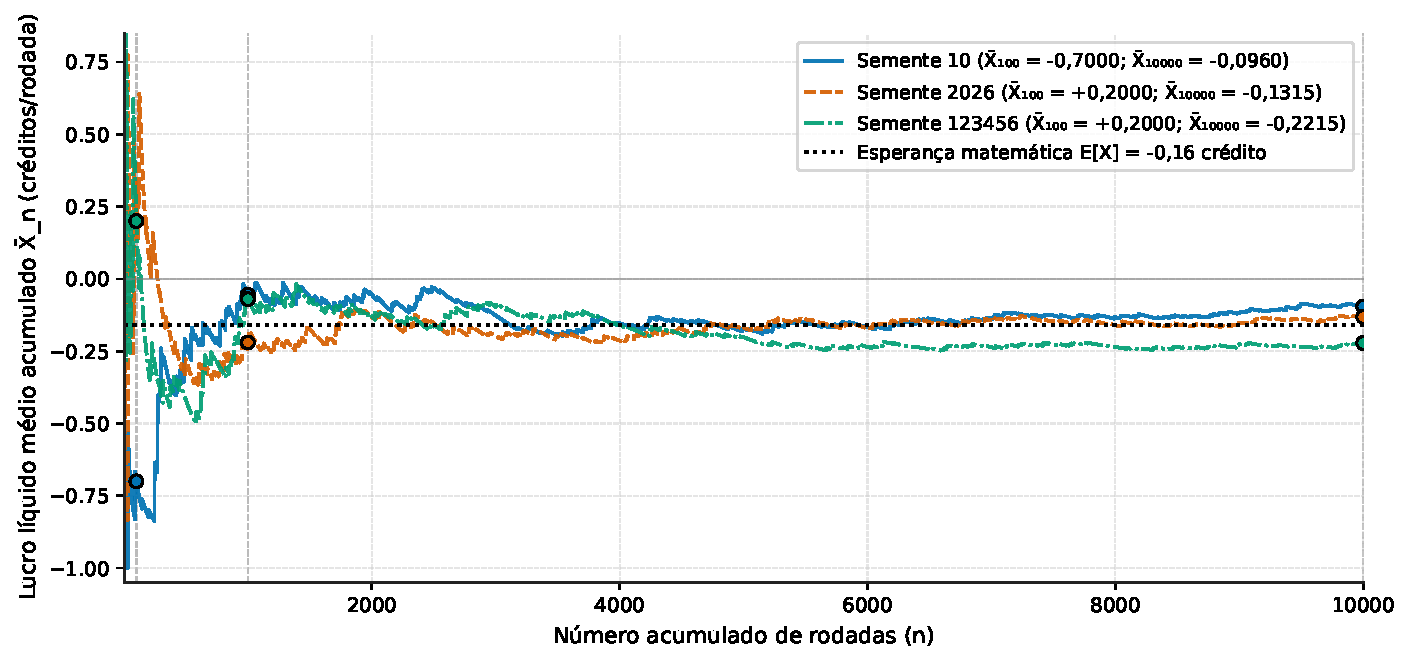
\includegraphics[width=0.95\textwidth]{resultados/graficos/fig03_e2_convergencia.pdf}
\caption{Trajetórias da média acumulada de lucro por rodada ($\bar{X}_n$) ao longo de $10.000$ rodadas para as sementes 10, 2026 e 123456 e referência horizontal $\mathbb{E}[X] = -0{,}16$ crédito.}
\label{fig:e2}
\begin{flushleft}
\scriptsize \textit{Fonte:} Elaboração própria com dados do Experimento 2.
\end{flushleft}
\end{figure}

\subsection{Experimento 3 -- O que acontece com um saldo limitado?}

Com semente única \textbf{42}, simularam-se $100$ participantes virtuais com saldo inicial $B_0 = 100$ créditos e parada em $500$ rodadas ou esgotamento ($B_t < 1$). Os resultados fecharam em: \textbf{ganho ($B_f > 100$) = 23,0\%} (23 pessoas), \textbf{empate ($B_f = 100$) = 2,0\%} (2 pessoas) e \textbf{perda ($B_f < 100$) = 75,0\%} (75 pessoas), somando $100{,}0\%$. O \textbf{esgotamento ($B_f = 0$) atingiu 67,0\%} de todos os participantes ($89{,}33\%$ dentre os que perderam). A \textbf{média dos saldos finais foi de 52,10 créditos} ($s = 93{,}51$, máximo $= 390$), enquanto a \textbf{mediana foi de 0,00 crédito} (Figura \ref{fig:e3}). Como a duração média das sessões foi abreviada pelo esgotamento para $\bar{\tau} = 339{,}90$ rodadas, não cabe usar $100 - 500(0{,}16) = 20$ como referência automática; pela Identidade de Wald, $100 - 339{,}90(0{,}16) = 45{,}62$ créditos.

\begin{figure}[H]
\centering
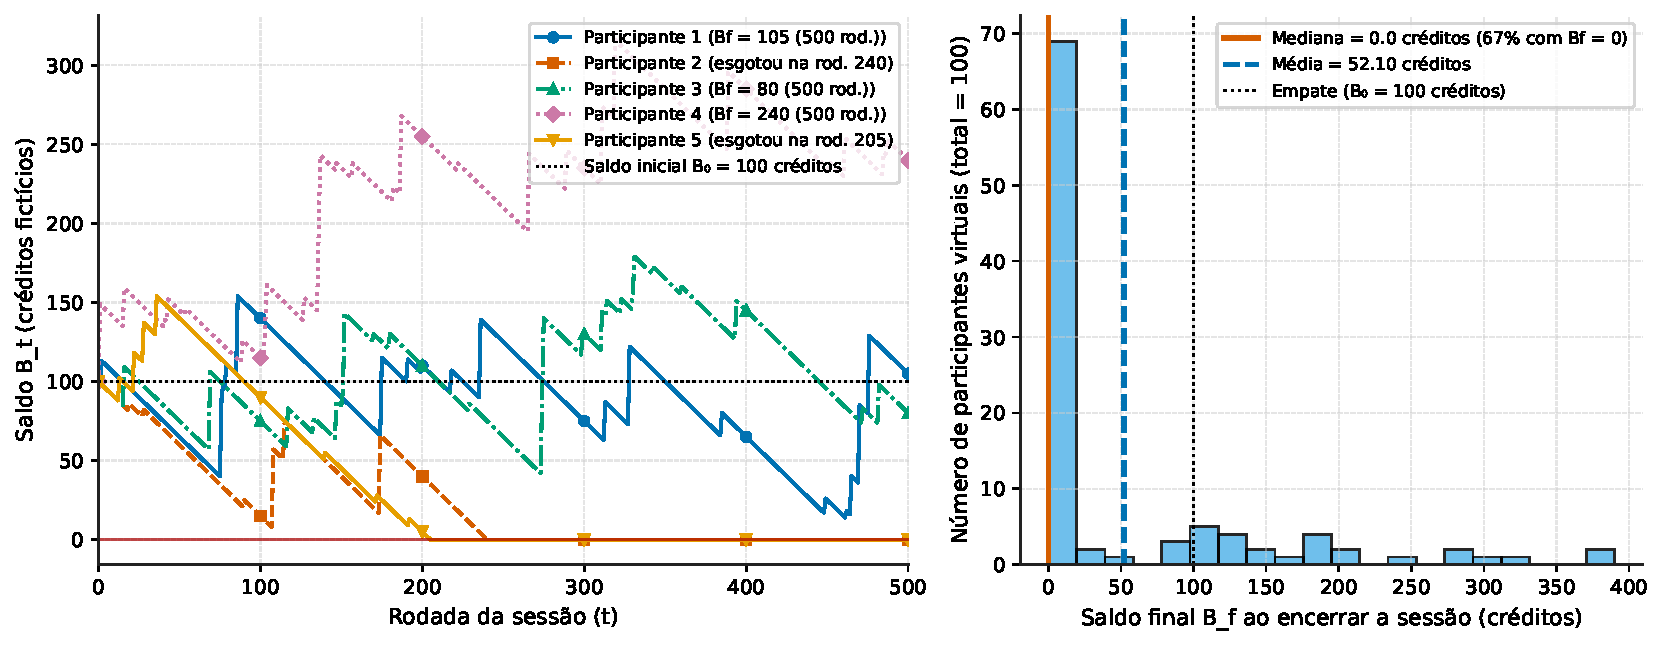
\includegraphics[width=0.98\textwidth]{resultados/graficos/fig04_e3_saldo_limitado.pdf}
\caption{Trajetórias do saldo $B_t$ dos cinco primeiros participantes virtuais sem seleção por desfecho (à esquerda) e distribuição dos saldos finais dos 100 participantes destacando média e mediana (à direita).}
\label{fig:e3}
\begin{flushleft}
\scriptsize \textit{Fonte:} Elaboração própria com dados do Experimento 3 (semente 42).
\end{flushleft}
\end{figure}

\subsection{Experimento 4 -- Depois de perder, aumenta a chance de ganhar?}

Nos $9.999$ pares consecutivos do Experimento 1, houve $412$ pares após prêmio ($17$ prêmios seguintes, proporção condicional $\widehat{\Pr}(G_{i+1}\mid G_i) = 4{,}1262\%$) e $9.587$ pares após perda ($395$ prêmios seguintes, $\widehat{\Pr}(G_{i+1}\mid G_i^c) = 4{,}1202\%$), somando $9.999$ pares ($412$ prêmios, $4{,}1204\%$; Figura \ref{fig:e4}). Ambos os grupos confirmam a referência teórica de independência ($\Pr(G_{i+1}) = 4{,}00\%$), refutando a \textbf{falácia do jogador}.

\begin{figure}[H]
\centering
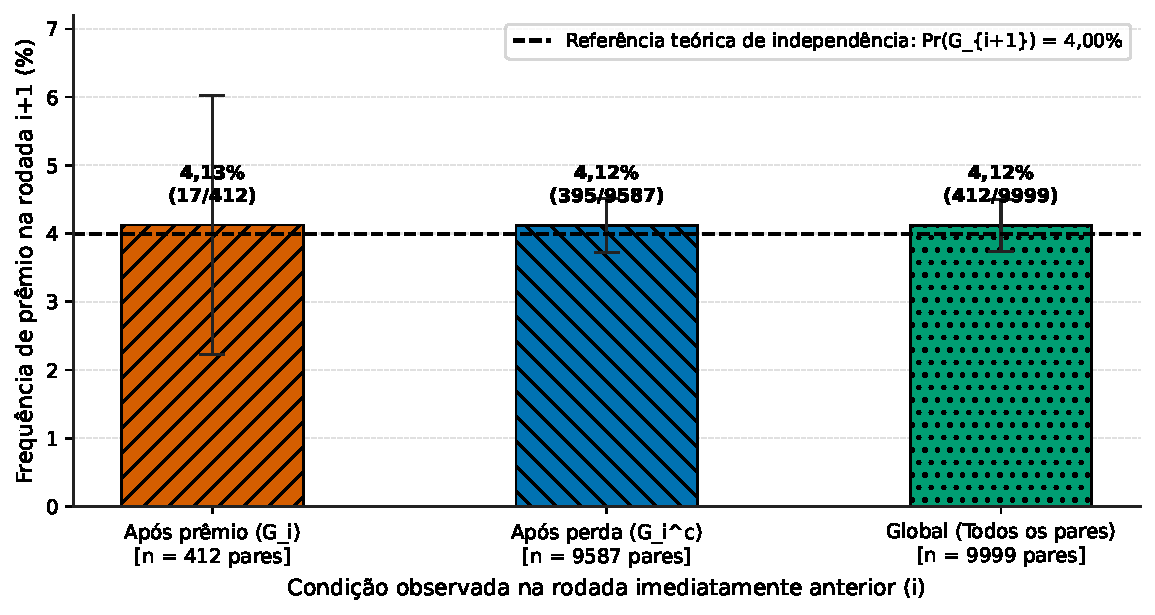
\includegraphics[width=0.78\textwidth]{resultados/graficos/fig05_e4_condicional.pdf}
\caption{Proporção observada de prêmio na rodada $i+1$ condicionada ao resultado da rodada anterior $i$ nos $9.999$ pares consecutivos do Experimento 4.}
\label{fig:e4}
\begin{flushleft}
\scriptsize \textit{Fonte:} Elaboração própria com dados do Experimento 4 (semente 2026).
\end{flushleft}
\end{figure}

\subsection{Experimento 5 -- Prêmios maiores tornam o jogo favorável?}

Aplicando a Tabela Prêmios $+10\%$ ($5{,}5; 11; 16{,}5; 27{,}5; 55$) aos mesmos $10.000$ sorteios do E1, a chance de prêmio manteve-se em $4{,}00\%$ teórica ($4{,}12\%$ observada), enquanto o RTP teórico subiu de $84{,}00\%$ para $\text{RTP}_{+10\%} = 1{,}10(0{,}84) = 92{,}40\%$ (observado de $86{,}85\%$ para $95{,}535\%$) e a esperança de lucro passou de $-0{,}160$ para $\mathbb{E}[X_{+10\%}] = -0{,}076$ crédito (observado de $-0{,}1315$ para $-0{,}04465$; Figura \ref{fig:e5}). Pagar mais melhora o retorno médio, mas não altera a frequência de prêmios nem torna a esperança positiva.

\begin{figure}[H]
\centering
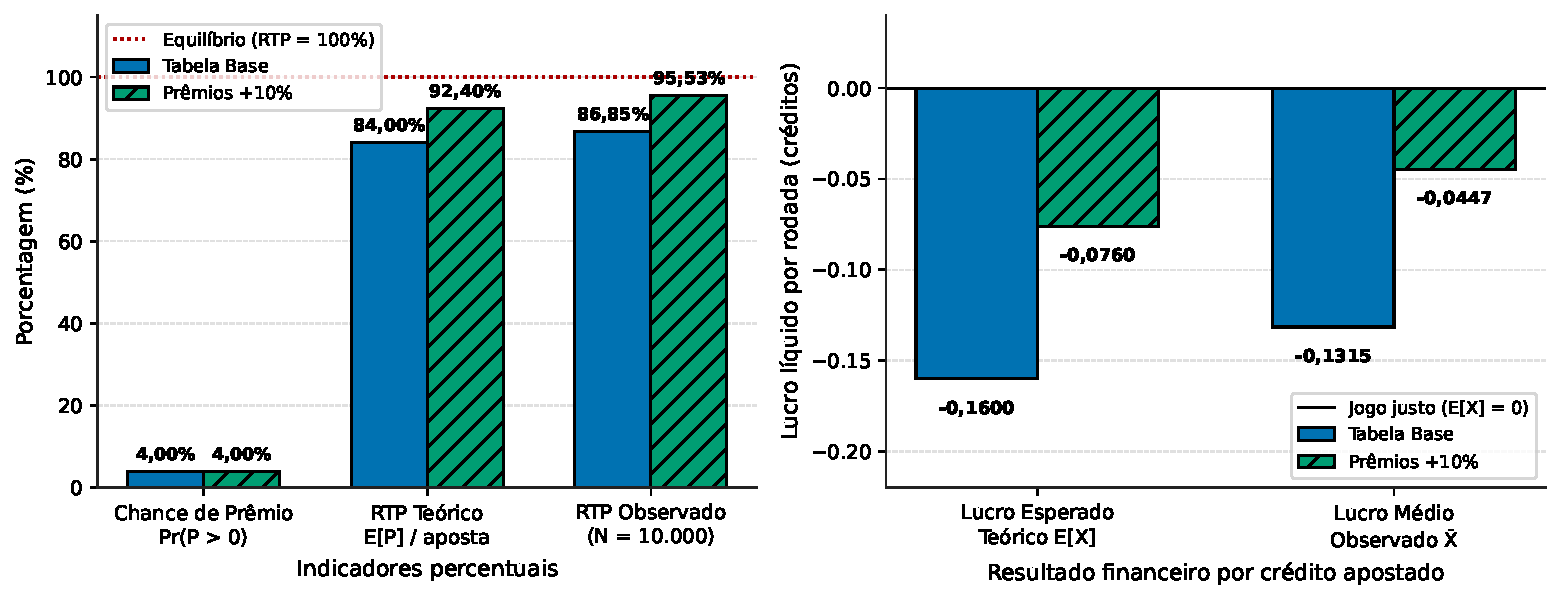
\includegraphics[width=0.96\textwidth]{resultados/graficos/fig06_e5_comparacao_tabelas.pdf}
\caption{Comparação entre a Tabela Base e a Tabela Prêmios $+10\%$ nos mesmos $10.000$ resultados do Experimento 1.}
\label{fig:e5}
\begin{flushleft}
\scriptsize \textit{Fonte:} Elaboração própria com dados do Experimento 5 (semente 2026).
\end{flushleft}
\end{figure}

\section{Da evidência à discussão crítica}

\textbf{1. Mecanismo e percepção.} A esperança negativa ($\mathbb{E}[X] = -0{,}16$) coexiste com ganhos ocasionais porque o desvio-padrão por rodada ($\sigma_X = 5{,}21$) é mais de 32 vezes superior ao módulo da perda média. Isso explica tanto as médias positivas temporárias em $n=100$ ($\bar{X}_{100}=+0{,}20$ no E2) quanto os $23\%$ de vencedores no E3, gerando viés de visibilidade nas redes sociais mentre $67\%$ esgotam seu saldo (mediana zero). Ademais, como mostram Newall et al. \cite{newall2020}, divulgar ``RTP de 84\%'' induz menor percepção de risco do que informar ``vantagem da casa de 16\%''.

\textbf{2. Renda e saúde.} Enquanto a simulação descreve propriedades de um modelo virtual, estudos empíricos documentam consequências reais: compressão da poupança e pressão sobre o crédito em famílias vulneráveis nos EUA (Baker et al. \cite{baker2024}), alto potencial danoso das máquinas rápidas (OMS \cite{oms2024}), prevalência agrupada de $15{,}8\%$ (IC 95\%: $10{,}7\%$--$21{,}6\%$) de jogo problemático entre adultos usuários de cassinos/rolos on-line (\textit{Lancet Commission} \cite{wardle2024}) e rastreamento nacional pela escala PGSI em $4.914$ participantes no LENAD III \cite{lenad2025} (distinguindo rastreamento populacional de diagnóstico clínico).

\textbf{3. Políticas e interesses.} A defesa de restrições severas (MP 1.394/2026 \cite{mp1394,ms2026}, ação da União \cite{richter2026}, IEPS \cite{ieps2025} e debates no Senado \cite{tvsenado2026}) ampara-se em fortes evidências sanitárias e nos fluxos financeiros observados pelo BCB \cite{bcb2024} e TCU \cite{tcu2026}, embora o custo social de R\$ 38,8 bi do IEPS \cite{ieps2025} deva ser lido considerando seus limites metodológicos (p.\ 33--35, extrapolação de revisão britânica \cite{ohid2023}). Já entre as críticas à proibição, os argumentos empresariais de ANJL/IBJR \cite{pontes2026} refletem interesses setoriais, mas o alerta técnico do Acórdão 1296/2026 do TCU \cite{tcu2026} sobre a dificuldade de fiscalizar e bloquear sites ilegais possui alta força probatória e exige coordenação estatal sobre meios de pagamento e publicidade.

\textbf{4. Responsabilidade profissional.} Profissionais de Sistemas de Informação devem rejeitar padrões manipulativos de interface (\textit{dark patterns}) e promover transparência algorítmica e acessibilidade, formulando ferramentas educativas que expliquem a matemática do risco sem prometer ganhos nem culpabilizar as pessoas afetadas.

\begin{thebibliography}{99}
\footnotesize
\bibitem{oms2024} WORLD HEALTH ORGANIZATION. \textit{Gambling}. 2 dez. 2024.
\bibitem{wardle2024} WARDLE, H. et al. The Lancet Public Health Commission on gambling. \textit{The Lancet Public Health}, v. 9, p. e950--e994, 2024.
\bibitem{lenad2025} UNIFESP; UNIAD. \textit{Caderno Temático LENAD III: jogos de aposta na população brasileira}. 2025.
\bibitem{baker2024} BAKER, S. R. et al. \textit{Gambling Away Stability: Sports Betting's Impact on Vulnerable Households}. NBER Working Paper 33108, nov. 2024.
\bibitem{newall2020} NEWALL, P. W. S.; WALASEK, L.; LUDVIG, E. A. Equivalent gambling warning labels are perceived differently. \textit{Addiction}, v. 115, n. 9, p. 1762--1767, 2020.
\bibitem{lei14790} BRASIL. \textit{Lei nº 14.790, de 29 de dezembro de 2023}.
\bibitem{mp1394} BRASIL. Congresso Nacional. \textit{Medida Provisória nº 1.394/2026}. Publicada em 25 set. 2026.
\bibitem{ms2026} BRASIL. Ministério da Saúde. \textit{Presidente Lula assina Medida Provisória que proíbe as bets no Brasil}. 25 set. 2026.
\bibitem{richter2026} RICHTER, A. Agência Brasil. \textit{Governo cobra na Justiça gastos do SUS com tratamento de apostadores}. 28 set. 2026.
\bibitem{pontes2026} PONTES, F. Agência Brasil. \textit{Associações de jogos acionam STF contra MP que proibiu apostas online}. 28 set. 2026.
\bibitem{bcb2024} BANCO CENTRAL DO BRASIL. \textit{Análise técnica sobre o mercado de apostas online no Brasil e o perfil dos apostadores}. Estudo Especial 119/2024; Nota Técnica 513/2024, set. 2024.
\bibitem{tcu2026} TRIBUNAL DE CONTAS DA UNIÃO. \textit{Acórdão 1296/2026 -- Plenário}. 19 maio 2026.
\bibitem{ieps2025} ROSA, D. et al. IEPS; FPSM; Umane. \textit{A saúde dos brasileiros em jogo}. Dez. 2025, 40 p.
\bibitem{ohid2023} OFFICE FOR HEALTH IMPROVEMENT AND DISPARITIES; PUBLIC HEALTH ENGLAND. \textit{Gambling-related harms: evidence review}. 2021/2023.
\bibitem{illowsky2023} ILLOWSKY, B.; DEAN, S. \textit{Introductory Statistics 2e}. OpenStax, 2023.
\bibitem{python_random} PYTHON SOFTWARE FOUNDATION. \textit{random --- Generate pseudo-random numbers}. Documentação do Python 3.12.7.
\bibitem{gc2021} GAMBLING COMMISSION. \textit{Return to player: how much gaming machines payout}. 2021.
\bibitem{ribas2025} RIBAS, N. M. et al. ``Jogo do Tigrinho'' e os perigos do Jogo patológico. \textit{Debates em Psiquiatria}, v. 15, e1393, 2025.
\bibitem{tvsenado2026} SENADO FEDERAL. TV Senado. \textit{Vício em bets: proibição das apostas online, saúde pública e endividamento das famílias}. 25 set. 2026.
\bibitem{pacete2024} PACETE, L. G. \textit{Conheça quem está por trás do Jogo do Tigrinho}. Forbes Brasil, 25 jun. 2024.
\end{thebibliography}

\end{document}
